\section{Convolutional Neural Network for Twitter sentiment}

\subsection{Network structure}

\begin{figure}[htb]
\centering
  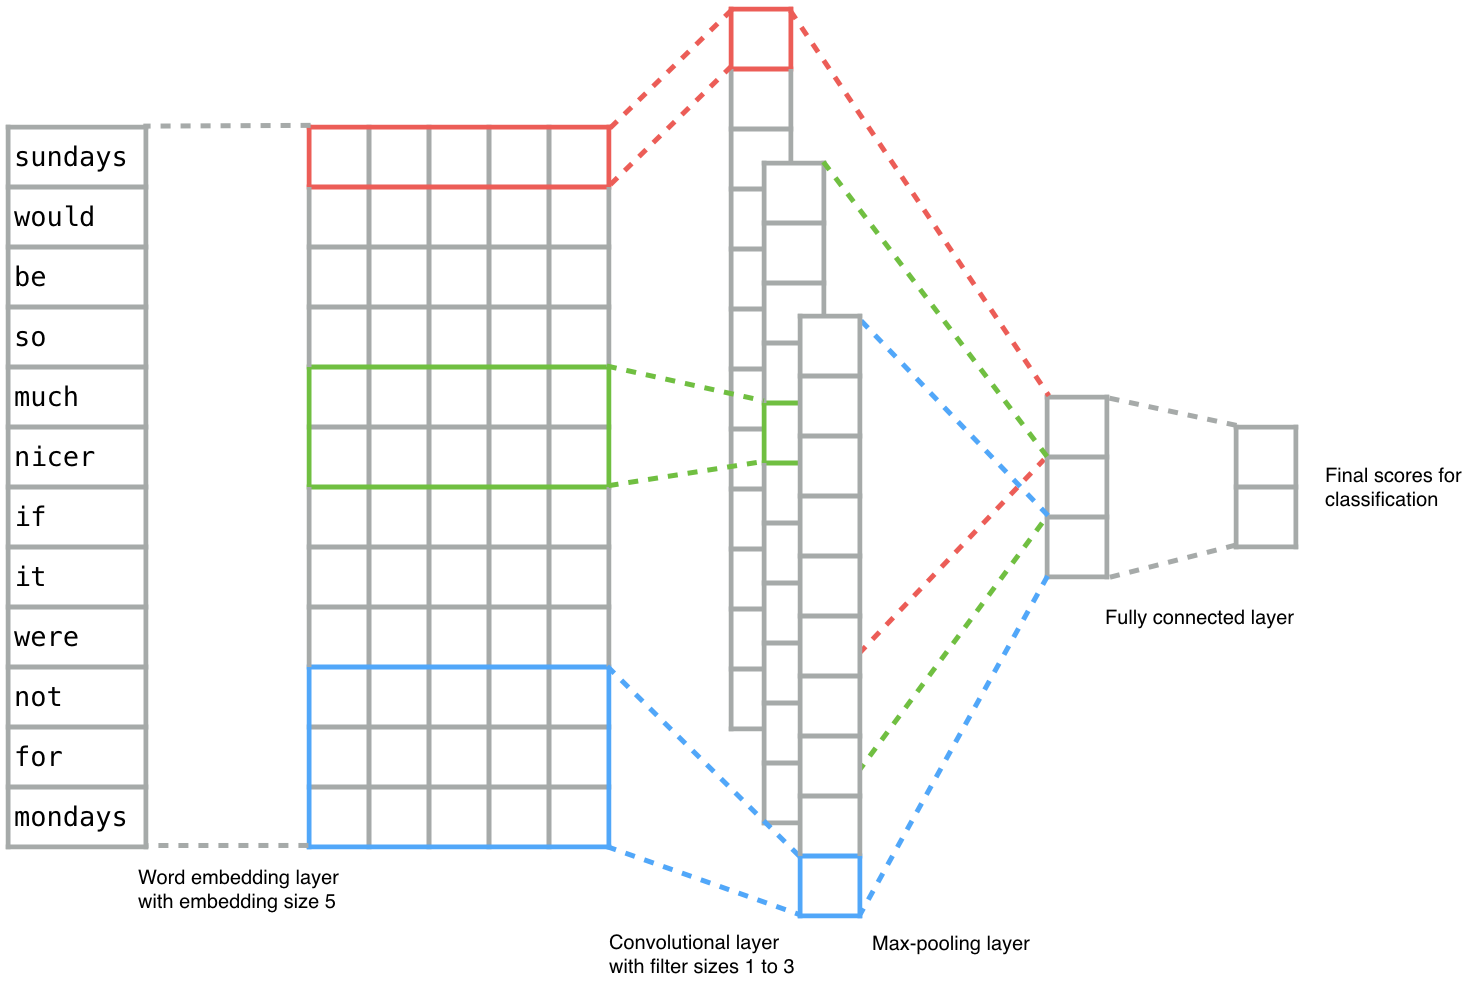
\includegraphics[width=0.8\linewidth]{figure/cnn.png}
  \caption{Structure of CNN}\label{fig.cnn}
\end{figure}

The structure of the CNN used in our term project is shown in Figure \ref{fig.cnn}. It is a simplification of the model used in \cite{kim2014}. Although this model has a minimalist design, it has most of the typical layers of a text-mining CNN: word embedding layer, convolutional layer, max-pooling layer, and fully-connected layer.

The first layer is the word embeddings, which is encoded as a weight matrix that is used as a lookup table. Each row of the weight matrix is a vector of size $k$ represents a unique word in the vocabulary. Given a sentence of length $n$, padded if necessary, each word is replaced by its corresponding vector and the sentence is converted to an output matrix that is a concatenation of all the embeddings. This output matrix is represented as
$$
\textbf{x}_{1:n} = \textbf{x}_1 \oplus \textbf{x}_2 \oplus \ldots \oplus \textbf{x}_n
$$
where $\textbf{x}_i \in \mathbb{R}^k$ is the embedding of the $i$-th word in the sentence, and $\textbf{x}_{i:ij} \in \mathbb{R}^{kj}$ is used to denote the sub-matrix from the $i$-th word to the $j$-th word.

The second layer is the convolutional layer. Given a window size $h$, this layer is encoded by a {\em filter} $\textbf{w} \in \mathbb{R}^{hk}$. When this filter is applied to the $h$-gram $\textbf{x}_{i:i+h-1}$ of the input sentence, a feature $c_i$ is generated by
$$
c_i = f(\textbf{w} \cdot \textbf{x}_{i:i+h-1} + b)
$$
where $b \in \mathbb{R}$ is bias and $f$ is the activation function such as rectifier. The filter slides over all the possible $h$-grams of the input sentence to produce a feature map
$$
\textbf{c} = (c_1, c_2, \ldots, c_{n-h+1})
$$ 
for $\textbf{c} \in \mathbb{R}^{n-h+1}$.

The next layer is the max-pooling layer. It is applied to the feature map produced by the convolutional layer to produce a single feature $\hat{c} = \text{max}(\textbf{c})$. Taking the maximum essentially picks the most important feature in the feature map, which is an effective way to deal with variable sentence length, because the special word for padding has 0s in all the dimensions in its word embedding. 

The last layer is a fully-connected layer. The $\hat{c}$ is the selected feature by a {\em single} filter, there're a number of filters with different window sizes. All the selected features from these filters are the input for this fully-connected layer, which uses softmax function to calculate the score for each class. 

\subsection{Regularization}

The purpose of regularization is to prevent overfitting or co-adaptation. Unlike \cite{kim2014}, only dropout is used to prevent co-adaptation, because according to \cite{zhang2015} the L2-norm constraint used in \cite{kim2014} generally has little effect on the end result, and we want to keep the network as simple as possible. The dropout is applied to the fully-connected layer of the CNN. It works by randomly setting a proportion $p$ of hidden units to 0 during learning. During testing, the dropout is disabled and the learnt weights are scaled down by $p$.

\subsection{Experiment}

\begin{table}[htb]
\centering
\begin{tabular}{| l | r |}
\hline
{\bf Hyperparameter} & {\bf Value}  \\ \hline
sentence length & 200 \\ \hline
word embedding size & 200 \\ \hline
filter window size & 1, 2 \\ \hline
number of filters per window size & 128 \\ \hline
dropout probability & 0.5 \\
\hline
\end{tabular}
\caption{Hyperparameters of CNN model}\label{tbl.cnn.param}
\end{table}

The dataset used in the experiments is from the Stanford Twitter Sentiment corpus \cite{go2009}, which consists of 1.6 million two-class machine-labeled tweets for training, and 498 three-class hand-labeled tweets for test. We composed a smaller training set of 25,000 positive and 25,000 negative examples from the original training set, and a smaller test set consists of all the 359 positive and negative examples from the original test set. The data is preprocessed to remove punctuations and other symbols like ``\#'' and ``@'', and to separate word contractions, e.g. ``don't'' to ``do not''. Each sentence is then tokenized by the {\tt TweetTokenizer} provided in Python NLTK \cite{bird2006} library and padded to 200 tokens as necessary. 

The CNN is implemented in TensorFlow, Google's deep learning library \cite{abadi2016}. The network structure is defined in Python, but the backend is implemented in C++, so the training and testing procedures run as C++ programs. The hyperparameters of the model are listed in Table \ref{tbl.cnn.param}. 

The skip-gram {\tt word2vec} model proposed in \cite{mikolov2013} is used for the word embedding layer. The size of the embeddings is 200. The embedding model is pretrained using a subset of the Google News data used in \cite{mikolov2013} that consists of 17 million words, with a vocabulary of 71,291 words. After plugged into the CNN, the parameters of the {\tt word2vec} model are set untrainable so it becomes a static lookup table. There're two reasons for fixing the parameters:
\begin{enumerate}
\item To reduce the number of parameters need to be learnt.
\item Tweets contain lots of noise, making the layer trainable exposes it to the noises, which may be counterproductive. \footnote{We did test the model with the embedding layer set trainable. The performance is slightly worse.}
\end{enumerate}
Because of this layer, the vocabulary of the CNN is determined by the {\tt word2vec} model, saved as a word-to-index dictionary. During data preprocessing, each word is converted to an index according to the dictionary. 

For the convolutional layer, there can be a number of a filters with different window sizes. In order to keep our model simple and small, only two windows sizes, 1 and 2, are used, and each window size has 128 filters. 

The model is trained with data batches of 128 tweets for 10 epochs. On a computer with 2.8GHz quad-core CPU and 16GB of memory, given pretrained {\tt word2vec} model, the CNN model can be trained and tested well under half an hour. We run the training and testing 20 times, and obtained an average accuracy of 79.60\%. Although this is not a very impressive performance, since our model has a very simple design and it is not optimized in any way, it still shows that there're lots of potentials in CNN.